\documentclass{article}
\usepackage[utf8]{inputenc}
\usepackage[a4paper, left=2.5cm, right=2.5cm, bottom=3cm, top=3cm]{geometry}
\usepackage{graphicx}
\graphicspath{ {./images/} }

\title{BDI and BAI Analysis Summary}
\author{Charles Mazof}
\date{September 4, 2022}

\begin{document}

\maketitle

\section*{Beck Depression Inventory (BDI)}

\bigskip
\bigskip

The Beck Depression Inventory is a measure of an individual's level of depression. Here we identify its relationship with various demographic measures, as well as with our measure of COVID-19 skepticism. 

\bigskip
\noindent
One-way ANOVAs were performed between each education group. Those without a college degree were significantly more depressed than those with a college degree or post-college degree.

\begin{table}[ht]
\centering
\caption{College Education vs Depression} \label{tab:title}
\begin{tabular}{llrrrrr}
  \hline
Group 1 & Group 2 & Estimate & Conf.low & Conf.high & P.adj & Sig \\ 
  \hline
No college degree & College degree & -2.80 & -4.63 & -0.96 & 0.00 & ** \\ 
No college degree & Graduate degree & -2.59 & -4.85 & -0.34 & 0.02 & * \\ 
College degree & Graduate degree & 0.20 & -2.08 & 2.49 & 0.98 & ns \\ 
   \hline
\end{tabular}
\end{table}

\bigskip
\bigskip
\noindent
The same comparison was done between income groups. Those in the lowest income brackets are more depressed than those who are in the higher income brackets.

\begin{table}[ht]
\centering
\caption{Income vs Depression} \label{tab:title}
\begin{tabular}{llrrrrr}
  \hline
Group 1 & Group 2 & Estimate & Conf.low & Conf.high & P.adj & Sig \\ 
  \hline
Less than \$50,000 & \$50,000 to \$100,000 & -2.15 & -4.05 & -0.26 & 0.02 & * \\ 
Less than \$50,000 & \$100,000 or more & -3.21 & -5.46 & -0.96 & 0.00 & ** \\ 
\$50,000 to \$100,000 & \$100,000 or more & -1.06 & -3.52 & 1.40 & 0.57 & ns \\ 
   \hline
\end{tabular}
\end{table}

\bigskip
\bigskip
\noindent
Race does not appear to significantly impact depression. 

\begin{table}[ht]
\centering
\caption{Race vs Depression} \label{tab:title}
\begin{tabular}{llrrrrr}
  \hline
Group 1 & Group 2 & Estimate & Conf.low & Conf.high & P.adj & Sig \\ 
  \hline
Chinese & Non Chinese Asian & -2.85 & -8.55 & 2.85 & 0.47 & ns \\ 
Chinese & White & 0.73 & -1.03 & 2.49 & 0.60 & ns \\ 
Non Chinese Asian & White & 3.58 & -2.04 & 9.19 & 0.29 & ns \\ 
   \hline
\end{tabular}
\end{table}

\pagebreak
\vspace*{\fill}

\noindent
A linear regression was performed between the BDI depression index and our measure of Covid Skepticism. No significant correlation was found.

\begin{table}[ht]
\centering
\caption{COVID-19 Skepticism vs Depression} \label{tab:title}
\begin{tabular}{rrrrr}
  \hline
 & Estimate & Std. Error & t value & Pr($>$$|$t$|$) \\ 
  \hline
(Intercept) & 11.6084 & 0.6131 & 18.93 & 0.0000 \\ 
  CovidSkepticism & -0.0111 & 0.0245 & -0.45 & 0.6515 \\ 
   \hline
\end{tabular}
\end{table}

\bigskip
\bigskip
\bigskip
\bigskip
\bigskip

{\centering 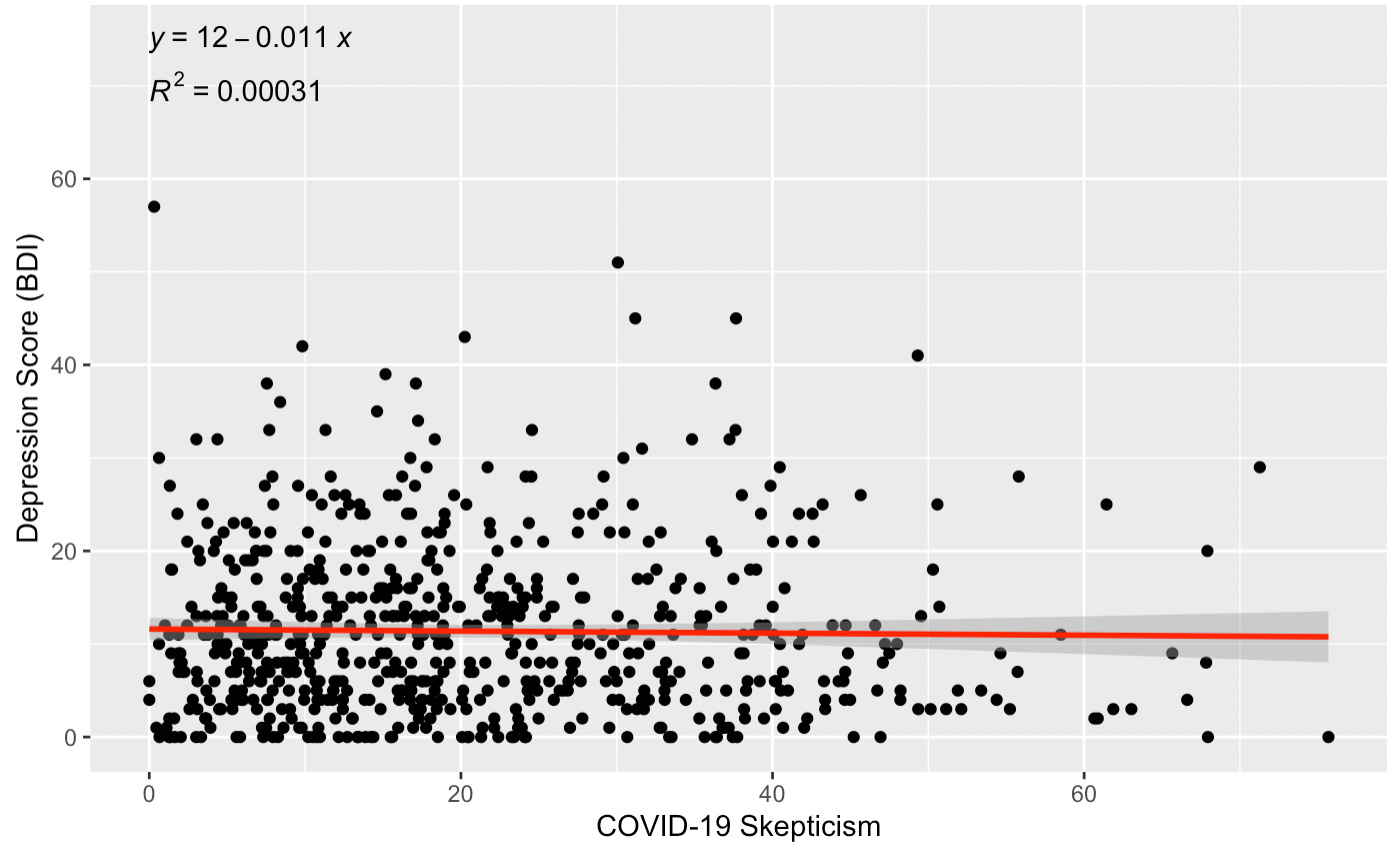
\includegraphics[scale=0.6]{BDICOVIDgraph.png} \par}

{\centering Figure 1: COVID-19 Skepticism vs Depression \par}

\vspace*{\fill}

\pagebreak

\vspace*{\fill}

\noindent
Lastly, younger people are more depressed.

\begin{table}[ht]
\centering
\caption{Age vs Depression} \label{tab:title}
\begin{tabular}{rrrrr}
  \hline
 & Estimate & Std. Error & t value & Pr($>$$|$t$|$) \\ 
  \hline
(Intercept) & 14.1500 & 0.2524 & 56.06 & 0.0000 \\ 
  DOB\_YEAR & -0.0949 & 0.0081 & -11.66 & 0.0000 \\ 
   \hline
\end{tabular}
\end{table}

\bigskip
\bigskip
\bigskip
\bigskip
\bigskip


{\centering 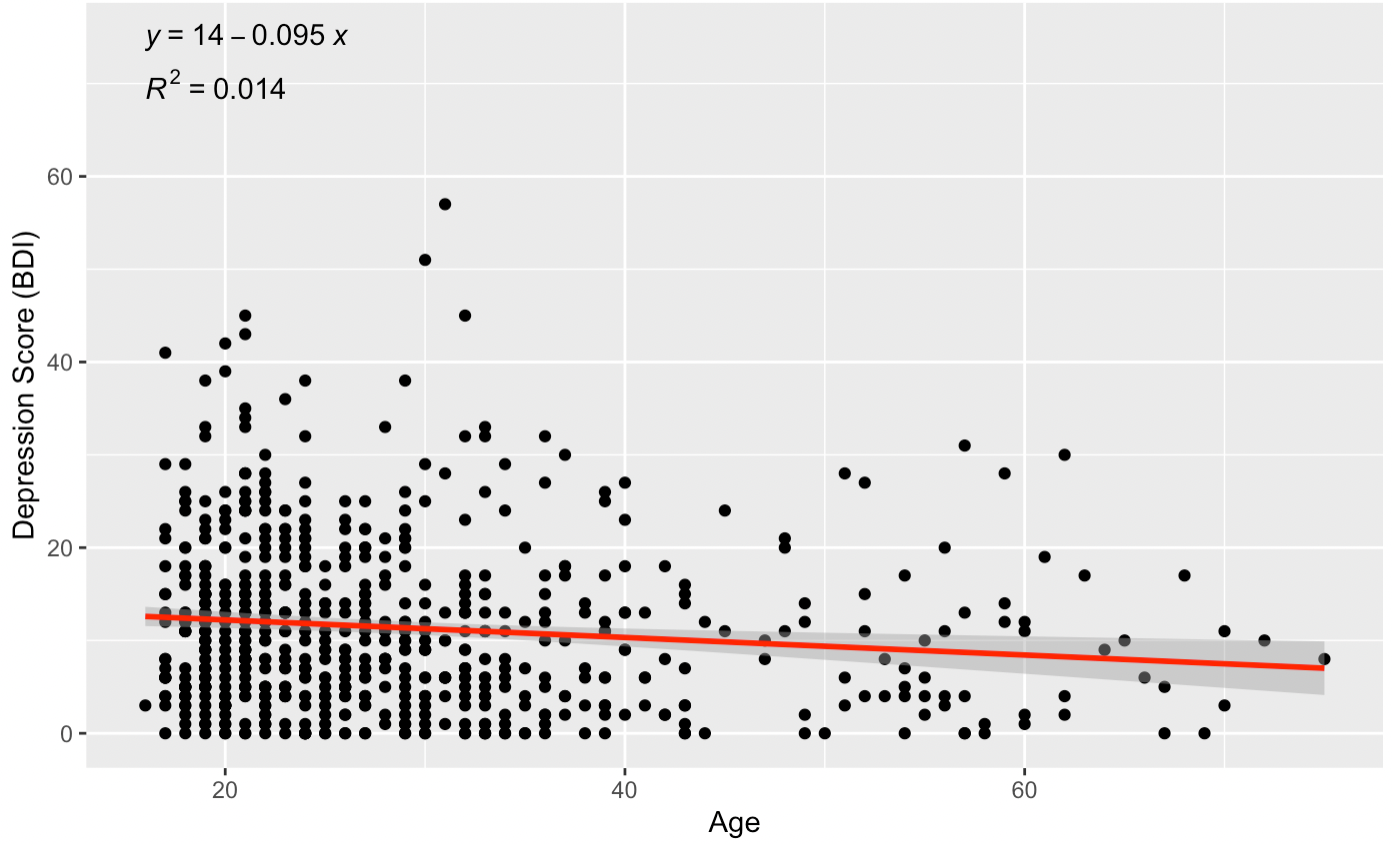
\includegraphics[scale=0.6]{BDIAGEgraph.png} \par}

{\centering Figure 2: Age vs Depression \par}

\vspace*{\fill}

\pagebreak

\section*{Beck Anxiety Inventory (BAI)}

\bigskip

The Beck Anxiety Inventory, similar to BDI, is a measure of an individual's anxiety level. We performed the same comparisons with as above.

\bigskip
\noindent
One-way ANOVAs were performed between each education group. Unsurprisingly, those without a college degree are more anxious than those with a college degree.

\begin{table}[ht]
\centering
\caption{Education vs Anxiety} \label{tab:title}
\begin{tabular}{llrrrrr}
  \hline
Group 1 & Group 2 & Estimate & Conf.low & Conf.high & P.adj & Sig \\ 
  \hline
No college degree & College degree & -2.63 & -4.79 & -0.48 & 0.01 & * \\ 
No college degree & Graduate degree & -2.06 & -4.71 & 0.59 & 0.16 & ns \\ 
College degree & Graduate degree & 0.58 & -2.10 & 3.26 & 0.87 & ns \\ 
   \hline
\end{tabular}
\end{table}

\bigskip
\bigskip
\noindent
There was no significant relationship between income and anxiety.

\begin{table}[ht]
\centering
\caption{Income vs Anxiety} \label{tab:title}
\begin{tabular}{llrrrrr}
  \hline
Group 1 & Group 2 & Estimate & Conf.low & Conf.high & P.adj & Sig \\ 
  \hline
Less than \$50,000 & \$50,000 to \$100,000 & -1.29 & -3.52 & 0.94 & 0.36 & ns \\ 
Less than \$50,000 & \$100,000 or more& -1.85 & -4.50 & 0.80 & 0.23 & ns \\ 
\$50,000 to \$100,000 & \$100,000 or more & -0.56 & -3.46 & 2.34 & 0.89 & ns \\ 
   \hline
\end{tabular}
\end{table}

\bigskip
\bigskip

\noindent
White people are significantly more anxious than Chinese people.

\begin{table}[ht]
\centering
\caption{Race vs Anxiety} \label{tab:title}
\begin{tabular}{llrrrrr}
  \hline
Group 1 & Group 2 & Estimate & Conf.low & Conf.high & P.adj & Sig \\ 
\hline
Chinese & Non Chinese Asian & -3.28 & -9.88 & 3.33 & 0.47 & ns \\ 
Chinese & White & 2.59 & 0.54 & 4.63 & 0.01 & ** \\ 
Non Chinese Asian & White & 5.86 & -0.65 & 12.37 & 0.09 & ns \\ 
   \hline
\end{tabular}
\end{table}

\vspace*{\fill}

\pagebreak

\vspace*{\fill}

\noindent
Regression analysis suggested that more anxious people were less skeptical about COVID-19, but this relationship did not meet our criteria for significance, $p < .05$.

\begin{table}[ht]
\centering
\caption{COVID-19 Skepticism vs Anxiety} \label{tab:title}
\begin{tabular}{rrrrr}
  \hline
 & Estimate & Std. Error & t value & Pr($>$$|$t$|$) \\ 
  \hline
(Intercept) & 12.1827 & 0.7141 & 17.06 & 0.0000 \\ 
  CovidSkepticism & -0.0554 & 0.0286 & -1.94 & 0.0528 \\ 
   \hline
\end{tabular}
\end{table}

\bigskip
\bigskip
\bigskip
\bigskip
\bigskip

{\centering 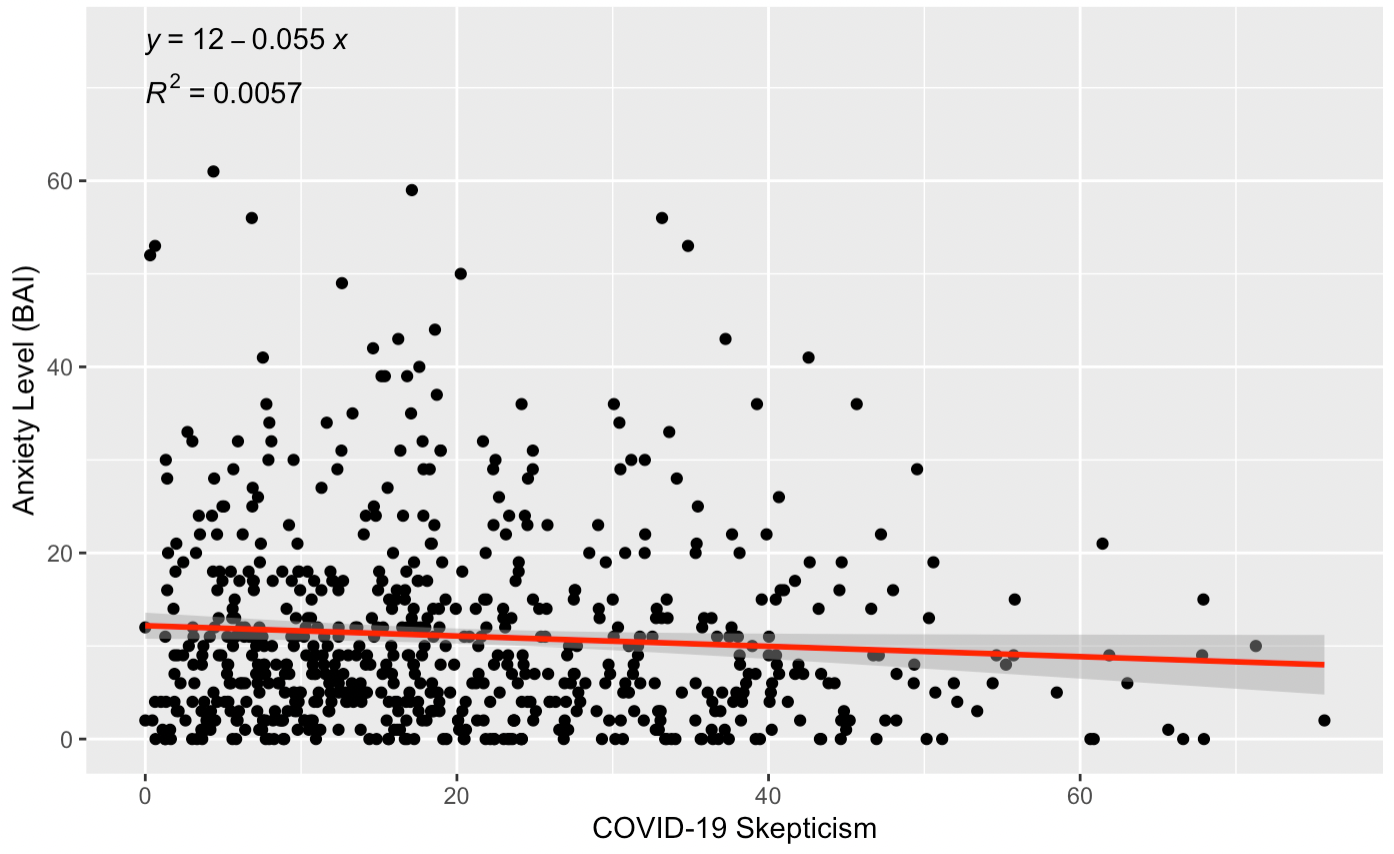
\includegraphics[scale=0.6]{BAICOVIDgraph.png} \par}

{\centering Figure 3: COVID Skepticism vs Anxiety \par}

\vspace*{\fill}

\pagebreak

\vspace*{\fill}

\noindent
People become less anxious as they get older.

\begin{table}[ht]
\centering
\begin{tabular}{rrrrr}
  \hline
 & Estimate & Std. Error & t value & Pr($>$$|$t$|$) \\ 
  \hline
(Intercept) & 13.9390 & 1.1211 & 12.43 & 0.0000 \\ 
  Age & -0.1002 & 0.0362 & -2.77 & 0.0058 \\ 
   \hline
\end{tabular}
\end{table}

\bigskip
\bigskip
\bigskip
\bigskip
\bigskip

{\centering 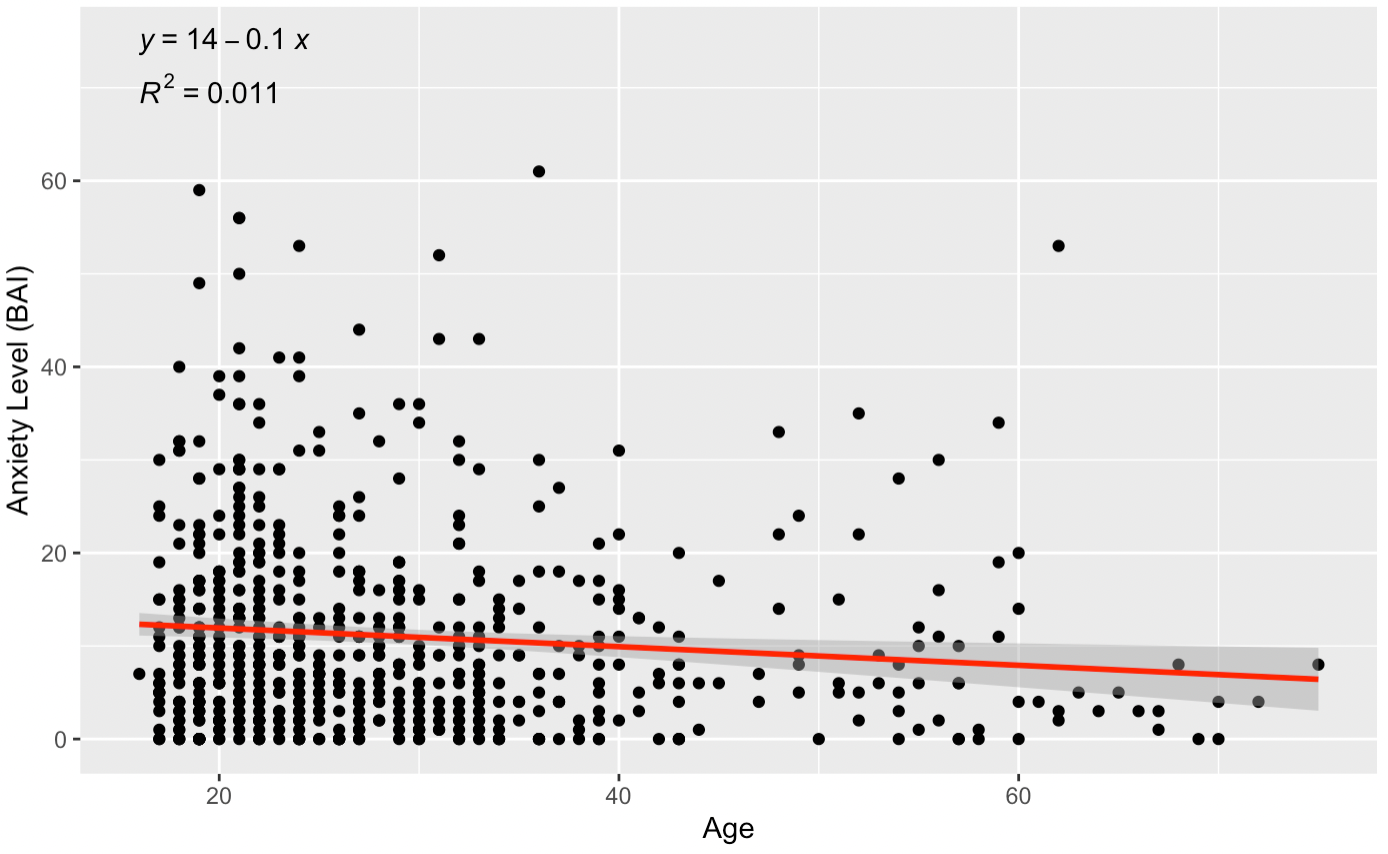
\includegraphics[scale=0.6]{BAIAGEgraph.png} \par}

{\centering Figure 4: Age vs Anxiety \par}

\vspace*{\fill}

\pagebreak

\vspace*{\fill}

\noindent
Finally, our anxiety and depression levels using this sample of participants are confirmed to be significantly correlated, R = 0.62. This value is surprisingly close to the literature value of R = 0.6.

\begin{table}[ht]
\centering
\begin{tabular}{rrrrr}
  \hline
 & Estimate & Std. Error & t value & Pr($>$$|$t$|$) \\ 
  \hline
(Intercept) & 2.8323 & 0.5206 & 5.44 & 0.0000 \\ 
  BDI score & 0.7221 & 0.0357 & 20.21 & 0.0000 \\ 
   \hline
\end{tabular}
\end{table}

\bigskip
\bigskip
\bigskip
\bigskip
\bigskip

{\centering 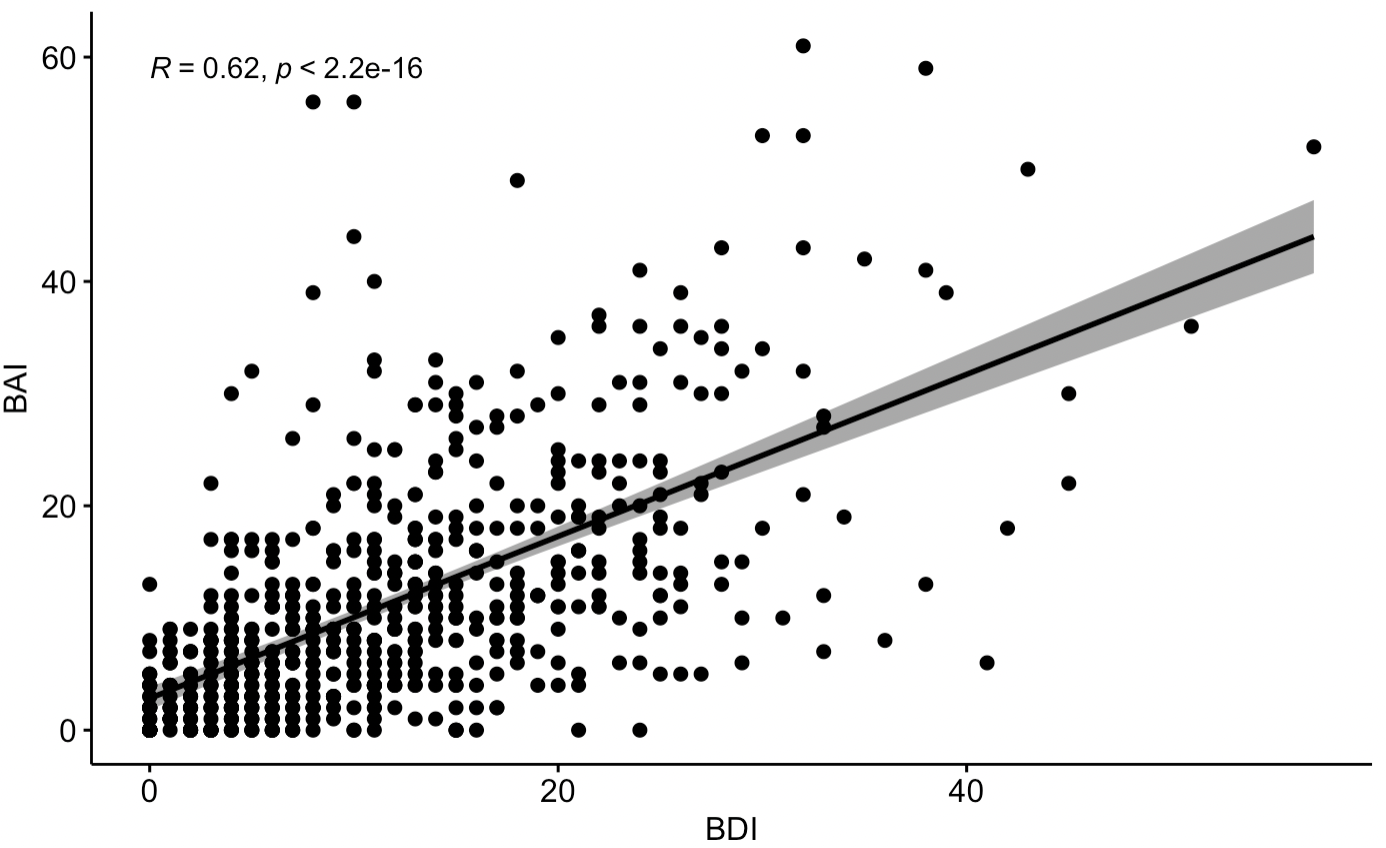
\includegraphics[scale=0.6]{BDIBAIcorr.png} \par}

{\centering Figure 5: BDI vs BAI \par}

\vspace*{\fill}

\end{document}
